%!TeX root=../main.tex
\فصل{نتایج}
\قسمت{مقدمه}
سیستم سنسور (سیستمی که وظیفه جمع‌آوری دیتا‌ها از سنسور‌ها و مخابره آن‌ها را دارد) اطلاعات را جمع‌آوری کرده و برای سیستم ایستگاه (سیستمی که وظیفه دریافت داده‌های ارسال شده و ارسال آن‌ها به رایانه را دارد) از طریق ماژول لورا مخابره می‌کند. در بخش ایستگاه انتظار می‌رود این اطلاعات بلافاصله دریافت شده و برای رایانه ارسال شود. در رایانه برنامه‌ای که برای همین منظور نوشته شده‌است، وظیفه دریافت اطلاعات ارسال شده از طریق \متن‌لاتین{USB} و ذخیره آن در دیتابیس را دارد. در این حالت انتظار می‌رود دیتا‌هایی که در نهایت برروی رایانه در دیتابیس ذخیره می‌شوند دقیقا مطابق با دیتا‌هایی باشد که دستگاه سنسور آن‌ها را جمع آوری و مخابره کرده است. همچنین انتظار می‌رود دستگاه ایستگاه قابلیت \متن‌لاتین{Plug \& Play} را داشته باشد به طوری که با اتصال دستگاه به \متن‌لاتین{USB} رایانه در صورت باز بودن برنامه این اتصال به طور خودکار شناسایی شده و برنامه در وضعیت متصل و آماده دریافت داده‌ها قرار بگیرد. 

\قسمت{تست برنامه دسکتاپ}
خروجی اطلاعات جمع‌آوری و مخابره شده توسط دستگاه بر روی رایانه و به کمک برنامه ساخته‌شده به همین منظور در سمت ایستگاه قابل‌مشاهده می‌باشد. جهت انجام بررسی‌های جزئی و ابتدایی به جهت پیش‌بینی وضعیت آب‌و‌هوایی برروی دیتاهای دریافتی، می‌توان از نمودار دیتاهای دریافتی که در تب \متن‌لاتین{Charts} برنامه قائل مشاهده است استفاده نمود. همچنین مشخصات و جزئیات آخرین دیتای دریافت شده نیز در تب \متن‌لاتین{Home} این نرم‌افزار قابل‌مشاهده است. تصاویری از محیط برنامه در  شکل \رجوع{fig:desktopApp} آمده است.

\begin{figure}[!h]
	\begin{subfigure}[b]{0.5\textwidth}
		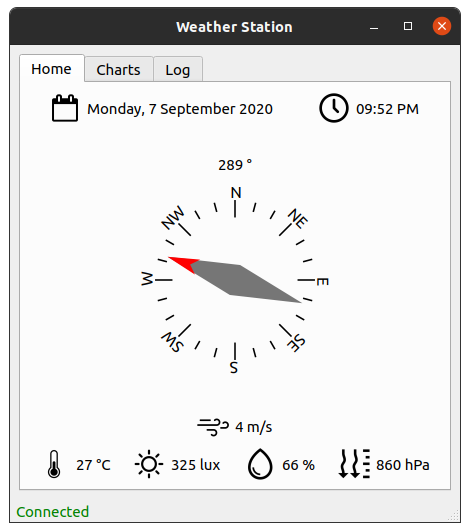
\includegraphics[width=\linewidth]{Assets/desktopAppHome.png}
		\caption{نمایش آخرین دیتاهای دریافتی برنامه در تب \متن‌لاتین{Home}.}
		\label{fig:desktopAppHome}
	\end{subfigure}
	\begin{subfigure}[b]{0.5\textwidth}
		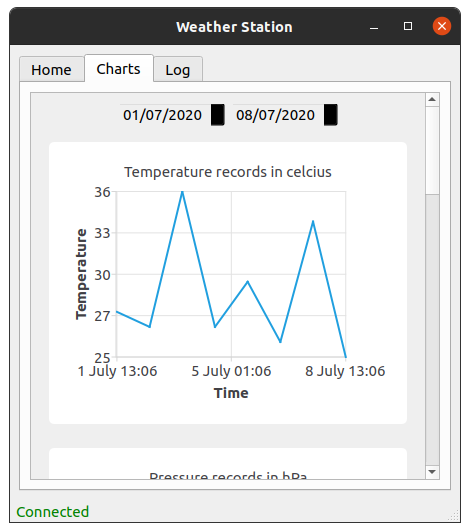
\includegraphics[width=\linewidth]{Assets/desktopAppCharts.png}
		\caption{نمایش نمودارهای اطلاعات دریافت شده در تب \متن‌لاتین{Charts}.}
		\label{fig:desktopAppCharts}
	\end{subfigure}
	\caption{تصاویر محیط برنامه دسکتاپ.}
	\label{fig:desktopApp}
\end{figure}

\noindent
همان طور که در تصویر \رجوع{fig:desktopApp} مشخص است در صورت اتصال دستگاه به رایانه در نوار وضعیت عبارت سبز رنگ \متن‌لاتین{Connected} (تصویر سمت راست) و در صورت عدم اتصال دستگاه به رایانه در نوار وضعیت عبارت قرمز رنگ \متن‌لاتین{Disconnected} (تصویر سمت چپ) درج می‌شود. همچنین در تب \متن‌لاتین{Charts} با انتخاب بازه تاریخ نمودار‌های مربوط به آن بازه به نمایش در خواهند آمد.

\قسمت{تست برد ماژول لورا}
در انجام تست‌های عملی مشخص شد برد مفید ماژول لورا علاوه بر وابستگی‌ای که به پارامترهای پهنای‌باند، ضریب پخش و توان دارد، به‌شدت به نوع آنتن وابسته است و نیازمند توجه ویژه‌ای به مسئله تطبیق امپدانس ترک‌های آنتن خروجی در طراحی بردمدارچاپی است. در نهایت طبق آزمایش صورت گرفته در منطقه مسکونی، در فرکانس 433 مگاهرتز، پهنای باند 20.8 کیلوهرتز، ضریب پخش 10، توان 20\متن‌لاتین{dBm} و یک آنتن دست‌­ساز، تا فاصله حدود 2 کیلومتری می‌توان دیتا‌های ارسالی را در سمت ایستگاه دریافت کرد. 


\قسمت{تست سنسور سنجش سرعت و جهت باد}
به دلیل در دسترس نبودن معیار دقیقی برای سنجش سرعت باد، نتیجه‌گیری در مورد دقت اندازه‌گیری سرعت باد اشتباه است اما با انجام آزمایشات متعدد دقت اندازه‌گیری جهت باد با سرعت متوسط و در دمای اتاق 4$\pm$ درجه به‌دست آمد. همچنین مشخص شد تغییر فاصله فرستنده و گیرنده‌های آلتراسونیک از یکدیگر و از زمین، عاملی مؤثر در تعیین دقت اندازه‌گیری و ماکسیموم سرعت قابل‌اندازه‌گیری است. به‌طوری‌که با نزدیک‌تر قرار دادن فرستنده و گیرنده (تا حداقل 4 سانتی‌متر) سرعت قابل‌اندازه‌گیری ماکسیموم و دقت اندازه‌گیری مینیموم می‌شود.


\vspace{1cm}
\بدون‌تورفتگی
{\درشت سورس‌کد تمامی پخش‌های پروژه به‌صورت متن‌باز در وبگاه \متن‌لاتین{GitHub} به نشانی زیر در دسترس است:}

\begin{latin}\noindent\large
	\href{https://github.com/jmdmahdi/Weather-Station}{https://github.com/jmdmahdi/Weather-Station}
\end{latin}

